\documentclass{standalone}
\usepackage{tikz}
\usetikzlibrary{patterns, positioning}
\usepackage[sfdefault]{ClearSans} %% option 'sfdefault' activates Clear Sans as the default text font
\usepackage[T1]{fontenc}

\begin{document}
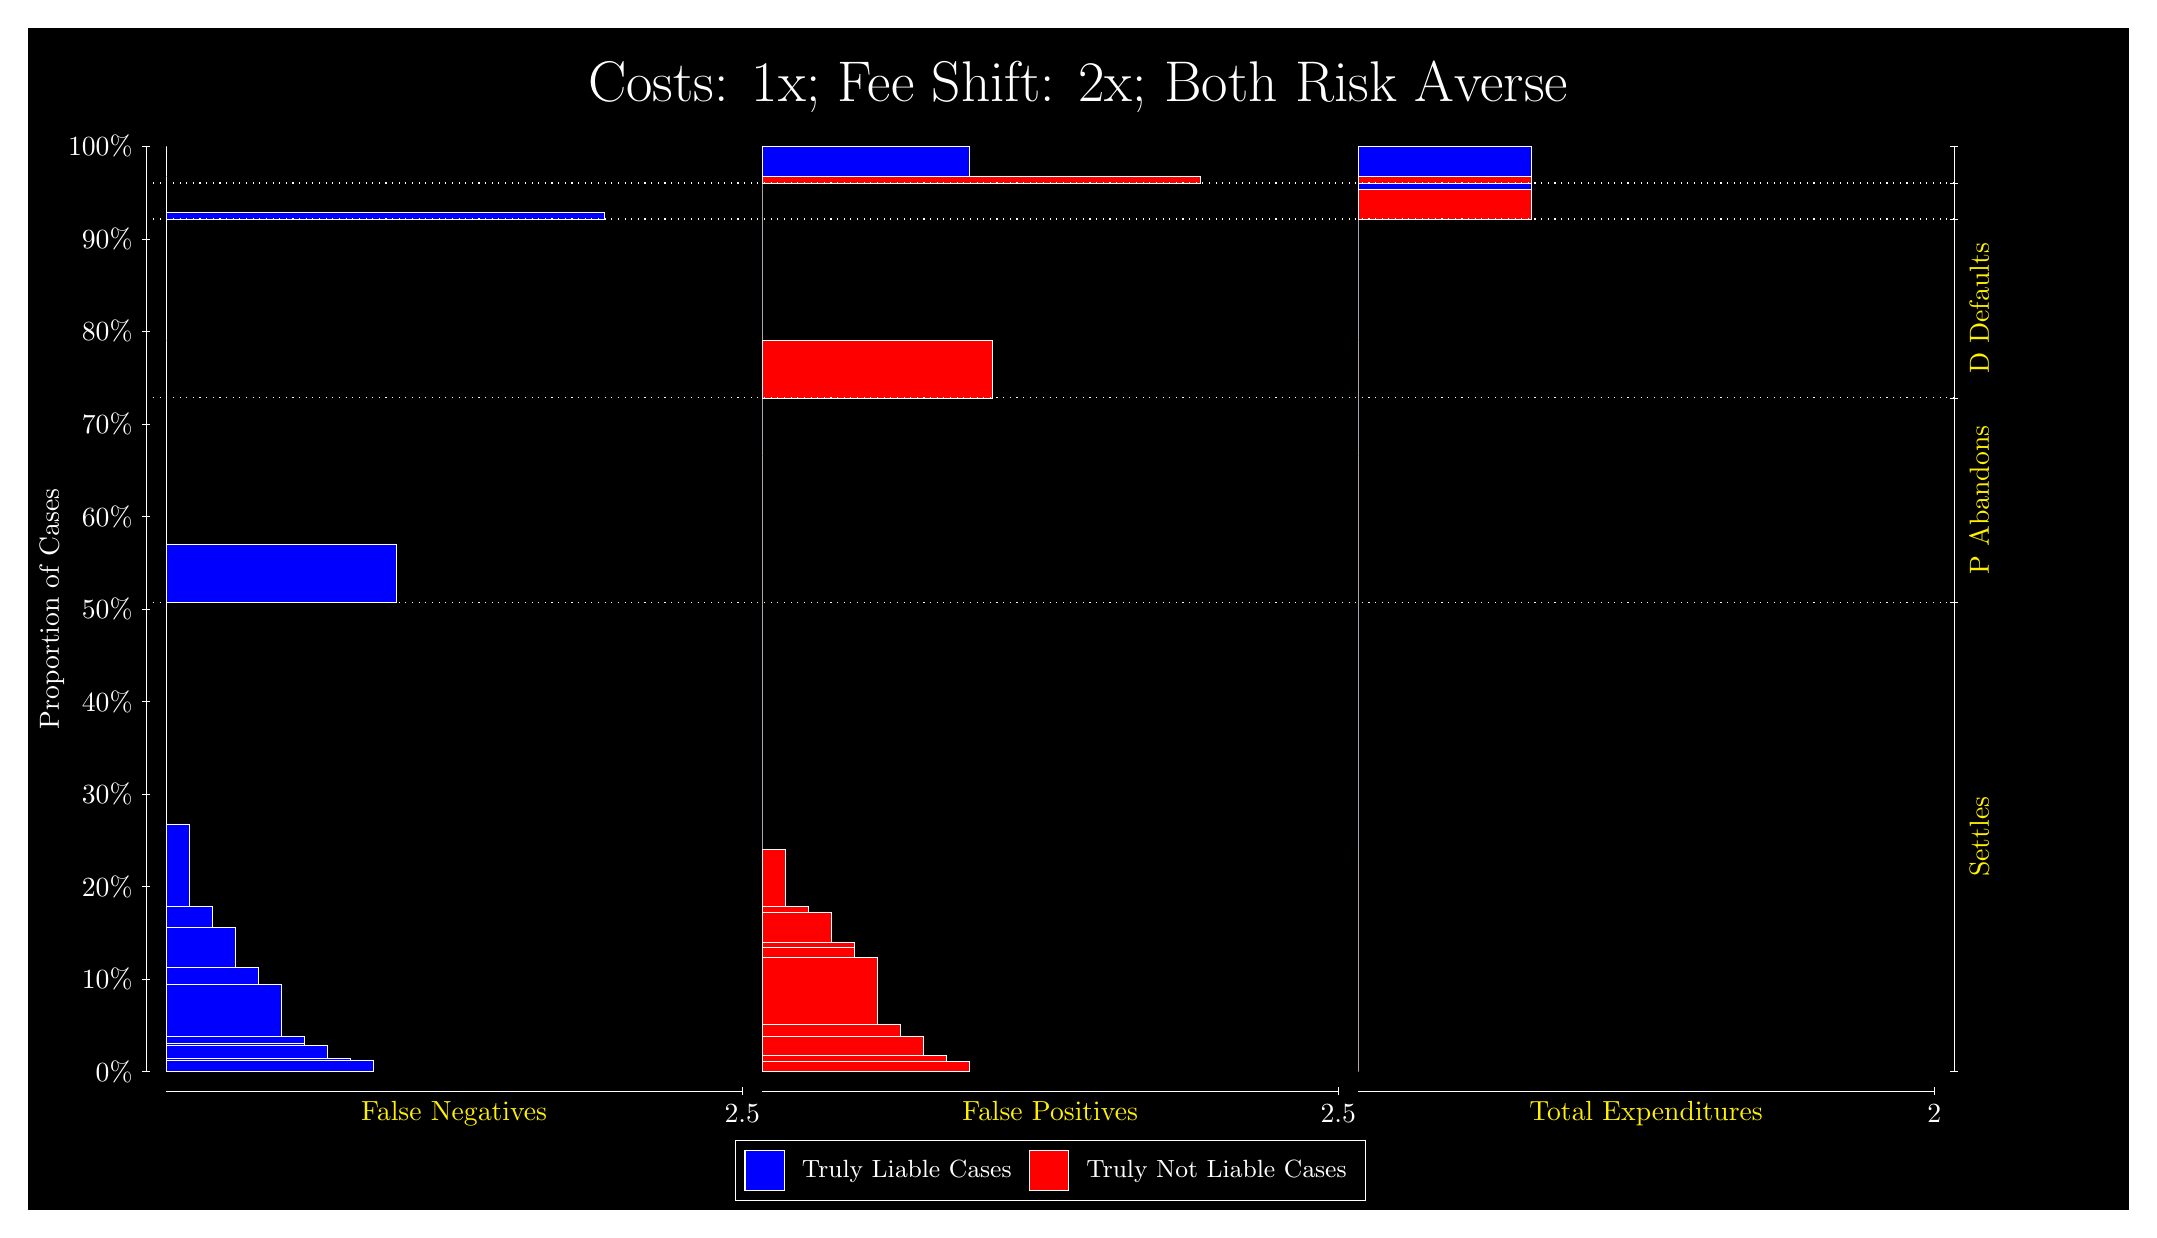
\begin{tikzpicture}
\draw[fill=black] (0,0) rectangle (26.667,15);
\draw[text=white] (0,13.5) rectangle (26.667,15) node[midway] {\huge Costs: 1x; Fee Shift: 2x; Both Risk Averse};
\draw[white, very thin] (1.5,1.75) -- (1.5,13.5);
\node[rotate=90, text=white, anchor=center] at (0.3, 7.625) {Proportion of Cases};
\draw[white, very thin] (1.45,1.75) -- (1.55,1.75);
\node[text=white, anchor=east] at (1.45, 1.75) {0\%};
\draw[white, very thin] (1.45,2.925) -- (1.55,2.925);
\node[text=white, anchor=east] at (1.45, 2.925) {10\%};
\draw[white, very thin] (1.45,4.1) -- (1.55,4.1);
\node[text=white, anchor=east] at (1.45, 4.1) {20\%};
\draw[white, very thin] (1.45,5.275) -- (1.55,5.275);
\node[text=white, anchor=east] at (1.45, 5.275) {30\%};
\draw[white, very thin] (1.45,6.45) -- (1.55,6.45);
\node[text=white, anchor=east] at (1.45, 6.45) {40\%};
\draw[white, very thin] (1.45,7.625) -- (1.55,7.625);
\node[text=white, anchor=east] at (1.45, 7.625) {50\%};
\draw[white, very thin] (1.45,8.8) -- (1.55,8.8);
\node[text=white, anchor=east] at (1.45, 8.8) {60\%};
\draw[white, very thin] (1.45,9.975) -- (1.55,9.975);
\node[text=white, anchor=east] at (1.45, 9.975) {70\%};
\draw[white, very thin] (1.45,11.15) -- (1.55,11.15);
\node[text=white, anchor=east] at (1.45, 11.15) {80\%};
\draw[white, very thin] (1.45,12.325) -- (1.55,12.325);
\node[text=white, anchor=east] at (1.45, 12.325) {90\%};
\draw[white, very thin] (1.45,13.5) -- (1.55,13.5);
\node[text=white, anchor=east] at (1.45, 13.5) {100\%};

\draw[white, very thin] (24.457,1.75) -- (24.457,13.5);
\draw[white, very thin] (24.407,1.75) -- (24.507,1.75);
\node[anchor=west] at (24.407, 1.75) {};
\draw[white, very thin] (24.407,7.7117) -- (24.507,7.7117);
\node[anchor=west] at (24.407, 7.7117) {};
\draw[white, very thin] (24.407,10.305) -- (24.507,10.305);
\node[anchor=west] at (24.407, 10.305) {};
\draw[white, very thin] (24.407,12.577) -- (24.507,12.577);
\node[anchor=west] at (24.407, 12.577) {};
\draw[white, very thin] (24.407,13.034) -- (24.507,13.034);
\node[anchor=west] at (24.407, 13.034) {};
\draw[white, very thin] (24.407,13.5) -- (24.507,13.5);
\node[anchor=west] at (24.407, 13.5) {};

\draw[white, very thin, fill=blue] (1.75,1.75) rectangle (4.3848,1.8873);
\draw[white, very thin, fill=blue] (1.75,1.8873) rectangle (4.092,1.9152);
\draw[white, very thin, fill=blue] (1.75,1.9152) rectangle (3.7993,2.0777);
\draw[white, very thin, fill=blue] (1.75,2.0777) rectangle (3.5065,2.112);
\draw[white, very thin, fill=blue] (1.75,2.112) rectangle (3.5065,2.1967);
\draw[white, very thin, fill=blue] (1.75,2.1967) rectangle (3.2138,2.8546);
\draw[white, very thin, fill=blue] (1.75,2.8546) rectangle (2.921,3.0703);
\draw[white, very thin, fill=blue] (1.75,3.0703) rectangle (2.6283,3.5792);
\draw[white, very thin, fill=blue] (1.75,3.5792) rectangle (2.3355,3.8471);
\draw[white, very thin, fill=blue] (1.75,3.8471) rectangle (2.0428,4.8859);
\draw[white, very thin, fill=red] (1.75,4.8859) rectangle (1.75,7.7117);
\draw[white, very thin, fill=blue] (1.75,7.7117) rectangle (4.6775,8.4415);
\draw[white, very thin, fill=red] (1.75,8.4415) rectangle (1.75,10.305);
\draw[white, very thin, fill=red] (1.75,10.305) rectangle (1.75,11.033);
\draw[white, very thin, fill=blue] (1.75,11.033) rectangle (1.75,12.577);
\draw[white, very thin, fill=blue] (1.75,12.577) rectangle (7.3123,12.657);
\draw[white, very thin, fill=red] (1.75,12.657) rectangle (1.75,13.034);
\draw[white, very thin, fill=red] (1.75,13.034) rectangle (1.75,13.115);
\draw[white, very thin, fill=blue] (1.75,13.115) rectangle (1.75,13.5);
\draw[white, very thin, fill=red] (9.3189,1.75) rectangle (11.954,1.8765);
\draw[white, very thin, fill=red] (9.3189,1.8765) rectangle (11.661,1.9558);
\draw[white, very thin, fill=red] (9.3189,1.9558) rectangle (11.368,2.2033);
\draw[white, very thin, fill=red] (9.3189,2.2033) rectangle (11.075,2.3549);
\draw[white, very thin, fill=red] (9.3189,2.3549) rectangle (10.783,3.2058);
\draw[white, very thin, fill=red] (9.3189,3.2058) rectangle (10.49,3.3324);
\draw[white, very thin, fill=red] (9.3189,3.3324) rectangle (10.49,3.3875);
\draw[white, very thin, fill=red] (9.3189,3.3875) rectangle (10.197,3.7668);
\draw[white, very thin, fill=red] (9.3189,3.7668) rectangle (9.9044,3.8489);
\draw[white, very thin, fill=red] (9.3189,3.8489) rectangle (9.6116,4.5758);
\draw[white, very thin, fill=blue] (9.3189,4.5758) rectangle (9.3189,7.7117);
\draw[white, very thin, fill=red] (9.3189,7.7117) rectangle (9.3189,9.5753);
\draw[white, very thin, fill=blue] (9.3189,9.5753) rectangle (9.3189,10.305);
\draw[white, very thin, fill=red] (9.3189,10.305) rectangle (12.246,11.033);
\draw[white, very thin, fill=blue] (9.3189,11.033) rectangle (9.3189,12.577);
\draw[white, very thin, fill=red] (9.3189,12.577) rectangle (9.3189,12.954);
\draw[white, very thin, fill=blue] (9.3189,12.954) rectangle (9.3189,13.034);
\draw[white, very thin, fill=red] (9.3189,13.034) rectangle (14.881,13.115);
\draw[white, very thin, fill=blue] (9.3189,13.115) rectangle (11.954,13.5);
\draw[white, very thin, fill=red] (16.888,1.75) rectangle (16.888,4.5758);
\draw[white, very thin, fill=blue] (16.888,4.5758) rectangle (16.888,7.7117);
\draw[white, very thin, fill=red] (16.888,7.7117) rectangle (16.888,9.5753);
\draw[white, very thin, fill=blue] (16.888,9.5753) rectangle (16.888,10.305);
\draw[white, very thin, fill=red] (16.888,10.305) rectangle (16.888,11.033);
\draw[white, very thin, fill=blue] (16.888,11.033) rectangle (16.888,12.577);
\draw[white, very thin, fill=red] (16.888,12.577) rectangle (19.083,12.954);
\draw[white, very thin, fill=blue] (16.888,12.954) rectangle (19.083,13.034);
\draw[white, very thin, fill=red] (16.888,13.034) rectangle (19.083,13.115);
\draw[white, very thin, fill=blue] (16.888,13.115) rectangle (19.083,13.5);
\draw[white, dotted] (1.5,7.7117) -- (24.457,7.7117);
\draw[white, dotted] (1.5,10.305) -- (24.457,10.305);
\draw[white, dotted] (1.5,12.577) -- (24.457,12.577);
\draw[white, dotted] (1.5,13.034) -- (24.457,13.034);
\draw[white, very thin] (1.75,1.5) -- (9.0689,1.5);
\node[text=yellow, anchor=north] at (5.4094, 1.5) {False Negatives};
\draw[white, very thin] (9.0689,1.45) -- (9.0689,1.55);
\node[text=white, anchor=north] at (9.0689, 1.45) {2.5};

\draw[white, very thin] (9.3189,1.5) -- (16.638,1.5);
\node[text=yellow, anchor=north] at (12.978, 1.5) {False Positives};
\draw[white, very thin] (16.638,1.45) -- (16.638,1.55);
\node[text=white, anchor=north] at (16.638, 1.45) {2.5};

\draw[white, very thin] (16.888,1.5) -- (24.207,1.5);
\node[text=yellow, anchor=north] at (20.547, 1.5) {Total Expenditures};
\draw[white, very thin] (24.207,1.45) -- (24.207,1.55);
\node[text=white, anchor=north] at (24.207, 1.45) {2};

\node[text=yellow, centered, rotate=90] at (24.777, 4.7308) {Settles};
\node[text=yellow, centered, rotate=90] at (24.777, 9.0084) {P Abandons};
\node[text=yellow, centered, rotate=90] at (24.777, 11.441) {D Defaults};



\draw (12.978300999999998,1.5) node[draw=none] (baseCoordinate) {};
\begin{scope}[align=center]
        \matrix[scale=0.5, draw=white, below=0.5cm of baseCoordinate, nodes={draw}, column sep=0.1cm]{
            \node[rectangle, draw, minimum width=0.5cm, minimum height=0.5cm, fill=blue] {}; &
            \node[draw=none, font=\small, text=white] (B) {Truly Liable Cases}; &
            \node[rectangle, draw, minimum width=0.5cm, minimum height=0.5cm, fill=red] {}; &
            \node[draw=none, font=\small, text=white] (B) {Truly Not Liable Cases}; \\
            };
\end{scope}

\end{tikzpicture}
\end{document}